\phantomsection\addcontentsline{toc}{section}{Introduction to Programs}%
\section*{Want to change the world with a job you love?\\
Get a computer science degree.}
Almost half of employers have open positions for computer science graduates, according to the National Association of Colleges and Employers (NACE). Nationally, average starting salaries top the list at \$72,173! Consistently in the top 5 for job satisfaction, computer science graduates are changing the world with their skills as software developers, cybersecurity analysts, web developers, project managers, and many other roles.


\subsection{Computer Majors at Charleston Southern University}
\begin{description}

	\item[Bachelor of Science (BS) Degree in Computer Science] This challenging track of studies emphasizes the computer languages and mathematical skills necessary to enter technical job markets. Jobs in these areas are typically high-paying. Our graduates are employed by the CIA, FBI, NASA, Pentagon, Naval Information Warfare Center (NIWC), Bank of America, Blackbaud, Blue Cross Blue Shield, Bosch, Disney, Intel, Texas Instruments, Microsoft, and many others.
	\item[Bachelor of Science (BS) Degree in Cybersecurity] The degree combines coursework in computer science, network security, criminal justice, and mathematics. It is targeted towards students wishing to enter the fields of network security or information analysis.
	\begin{minipage}[][][t]{0.69\linewidth}
		\vspace{3pt}
		\item[Bachelor of Arts (BA) Degree in Applied Computing] This program is a highly flexible and challenging major for computer-related professions in business, the visual and musical arts, religious service, public service, health care, etc. Choose between concentrations in business, graphic arts, or cybersecurity.
		\item[Bachelor of Technology (BT) Degrees in Computer Science or Cybersecurity] This online degree is a special program for individuals with approved Associate Degrees. Such individuals typically transfer their Associate degrees intact with almost no loss of credits so that they can complete custom-fit four-year degrees in about two years.\vspace{0.5em}
	\end{minipage}
	\begin{minipage}[][][t]{0.3\linewidth}%
		\hfill
		% Flip the image horizontally
		\scalebox{-1}[1]{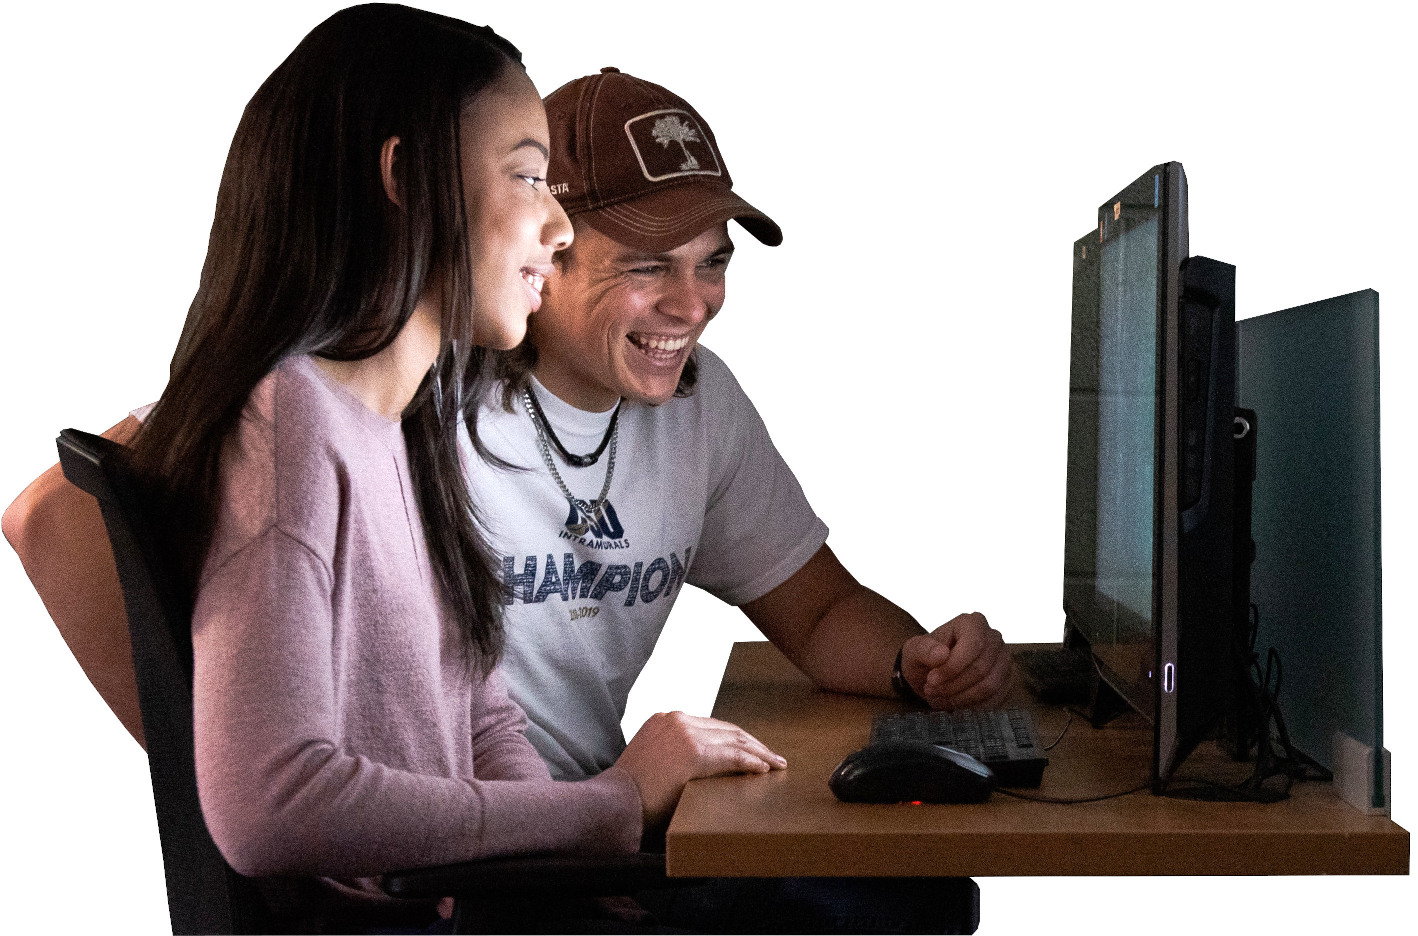
\includegraphics[width=0.95\textwidth]{SmilingTeamwork}}%
	\end{minipage}
\end{description}

\subsection{Faculty}
\begin{description}[leftmargin=0px]
	\item[Dr. Sean Hayes] Ph.D. Computer Science, Vanderbilt University: award-winning researcher in mobile user-interface design.
	\item[Dr. Yu-Ju (Joseph) Lin] Ph.D. Electrical \& Computer Engineering, University of Florida: Networking researcher and author.
	\item[Dr. Valerie Sessions] Ph.D. Computer Science \& Engineering, USC: Information Quality researcher, award-winning author.
	\item[Dr. Paul West] Ph.D. Computer Science, Florida State: Architecture researcher/author. Google Android, SPAWAR, Atlantic.
	\item[Prof. Julie Henderson] M.S. Computer Science, Clemson University: IBM patent holder, GIAC Certified Forensic Examiner.
	\item[Prof. Mike O’Neill] M.S. Health Physics, Georgia Institute of Technology: Database and network admin with a security focus.
	\item[Prof. Jim Roberts] M.C.S. Computer Science, Texas A \& M: Satellite research, development, and operations.
	\item[Prof. Fred Worthy] M.A.T. Mathematics, Colorado State University:  From NASA. Worked on the first lunar landing.
\end{description}

\subsection{Our Unique Environment}
\begin{description}
	\item[Mission] Our mission is to incubate technically excellent, highly ethical, can-do computer professionals who will learn, lead, and serve from a Biblical worldview. To this end, we focus on the unchanging fundamentals of computer science and emphasize Christian character and ethical behavior.
	\item[Over-the-shoulder Teaching] Involved students learn best. Consequently, most courses are taught in the lab with each student fully engaged with the computer while the subject is being taught. The faculty typically “coach” over the shoulder as opposed to delivering only standard lectures. This teaching method gives our graduates an “edge” in the workplace.
	\item[Small Class Size] Computer classes do not exceed 24 students per class and are usually smaller.
	\item[Emphasis on Teamwork] Teamwork is critical to success in the information technology workplace. For this reason, our courses stress teamwork in-class assignments. Students learn to apply team dynamics to accomplish complex tasks.
	\item[Focus on the Real World] Our goal is to produce well-rounded graduates who can succeed in the real world.  To this end, each student must complete a year-long, senior project under the direction of a mentor and defend it orally. During the project, each student must demonstrate independent research, self-learn the skills needed, then design and complete the project to the customer’s satisfaction.  Each must also pass a comprehensive exit exam.
	\item[Graduate Program] Students can earn a master’s degree in CS with only one additional year of school.
	\item[Web Site] \href{https://www.charlestonsouthern.edu/academics/college-of-science-and-mathematics/}{charlestonsouthern.edu/academics/college-of-science-and-mathematics/}
\end{description}